% (c) 2020 Stefan Antonowicz
% Based off of tex found at https://github.com/ludus-leonis/nipajin
% This file is released under Creative Commons Attribution-NonCommercial-ShareAlike 4.0 International License.
% Please do not apply other licenses one-way.

\renewcommand{\yggEquipment}{%
  \mychapter{Equipment}{equipment}
}

\renewcommand{\yggEquipmentText}{%

\mysection{Burden}{gear-burden}

  \ed{To the best of my knowledge, Significant and Insignificant items come from Logan Knight's "In Corpathium"}

  Encumbrance; hindrance; weight; load - whatever you call it, it seems that games have been trying to figure out how to limit how much weight an Adventurer can carry since Gygax first put pencil to paper.  Too much and it feels like algebra homework, too little and you have munchkins bristling with dozens of axes.  

  Hopefully this is the sweet spot.

  In the Totality of Ygg, Burden is broken down into \mybold{Significant} and \mybold{Insignificant} Items.  

  \myhighlight{Insignificant Items}{equipment-insignificant-items}

  You can carry as many Insignificant Items as you want as long as you can tell the Arbiter where they are i.e. "I've got the 11 weird rocks we've found at the bottom of my backpack, the amulet is tied to my belt, and I stowed the matches in my pocket".  Be reasonable, and the Arbiter has final say.

  \myhighlight{Significant Items}{equipment-significant-items}

  The number of Significant Items you can carry depends on your \MAX \VIG +2 i.e. if you have a d12 \VIG, you can carry 14 Significant Items. \mylink{Pooka}{species-pooka} and \mylink{Night Children}{species-night-child} don't get the +2 bonus, because they're Tiny - they can only carry their \MAX \VIG items.

  If you try to carry more than your \MAX, you're Morbidly Encumbered and you can only shuffle around (no Fight, no Guard, etc),  Some examples of Significant Items:

  \mybullet {
    \item Some Gear counts as a Significant Item (see list below)
    \item If a weapon does d4 damage, it counts as 1/2. 1 handed weapons count as 1.  2 handed weapons count as 2. 
    \item Light armor and shields count as 1 each. Medium armor counts as 2.  Heavy Armor counts as 3.
    \item 4kg worth of coins counts as 1. A person counts as ~100kg (25 Significant Items), but Pooka and Night Children are only 15
    \item Certain things you might try to pick up while adventuring - a carpet, an anvil, a millstone, etc. will be worth a certain number of Significant Items as determined by the Arbiter.  For example, a large carpet might have a Burden of 12 - meaning that you will need 12 Significant Item slots (collectively) to carry the carpet out of the dungeon at a shuffling pace.
    \item Finally, certain effects on you might fill your Significant Item slots (priests of the Corpulent One, for example, might need to be obese to be able to use their special powers, and that obesity might equal 2 or 3 Significant Items)
  }

  \example {
    Andre Preneur, assassin for hire, carries out his contracts with two daggers sheathed in a small poison-filled bladder on his back (1) and carries a Grappling Hook (1) and 25m of rope (1).  His Burden is 3.
    ~\\


    Balthazar the Breathtaking carries a knave's sword (1) with a bandolier of 4 daggers (1. The bandolier halves the value of the daggers).  He's got a bunch of shrunken heads tied to his belt and to the hilt of his sword with spell incantations written on them, but these are Insignificant Items - so his Burden is 2.
    ~\\

    The Nightie Knight uses a longsword (1), a shield (1), and wears Heavy armor (which has a Burden of 0 because she has the Sellsword Virtue \mylink{Second Skin}{sellsword-virtue-second-skin}).  She carries a Strongbow on her back (2) with a quiver on her hip (1).  Her Burden is 5.
  }


\newpage
\end{multicols}

\mysection{Weapons}{gear-weapons}

  \example{
    \mylist {
      \item \mybold{Hard:}  Hard Weapons use \VIG for Fight checks
      \item \hrulefill
      \item \mybold{Fast:}  Fast Weapons use \DEX for Fight checks
      \item \hrulefill
      \item \mybold{Type:}  The type or class of the weapon: Stabbing, Chopping, or Bashing
      \item \hrulefill
      \item \mybold{Brawl:}  Brawl Weapons can only be used on Monsters Close to you.
      \item \hrulefill
      \item \mybold{Throw:}  Throw Weapons can be used on Monsters Close to you, or thrown Nearby
      \item \hrulefill
      \item \mybold{Shoot:}  Shoot Weapons can target foes Nearby to Distant (but not Close).
      \item \hrulefill
      \item \mybold{Burden:}  Two handed weapons have a Burden of 2; weapons that do d4 damage have a Burden of ½
    }
  }



  \mytable{X X X X X X X}{
    \thead{} &\thead{Damage} & \thead{Hands} & \thead{Means} & \thead{Type}  & \thead{Range} & \thead{Traits} \\
  }{
    Bow &  d6  & 2h & Fast & Stabbing & Shoot  &  \\
    Club &  d4  & 1h & Hard & Bashing & Brawl & \\
    Dagger &  d4  & 1h & Fast & Stabbing & Throw & \\
    Hand Axe &  d4  & 1h & Hard & Chopping & Throw & \\
    Knave's Sword &  d8  & 1h & Fast & Stabbing & Brawl &  \\
    Longsword &  d8  & 1h & Hard & Chopping & Brawl &  \\
    Mace &  d8  & 1h & Hard & Bashing & Brawl & \\
    Military Pick &  d10  & 2h & Hard & Stabbing & Brawl & \mylink{Brutal}{gear-weapon-brutal}  \\
    Polearm &  d10  & 2h & Hard & Chopping & Brawl & \mylink{Rend}{gear-weapon-rend} and \mylink{Brace}{combat-tactical-maneuver-brace} \\
    Quarterstaff &  d6  & 2h & Fast & Bashing & Brawl & \\
    Shortsword &  d6  & 1h & Fast & Chopping & Brawl &  \\
    Sling &  d4  & 1h & Fast & Bashing & Shoot & \\
    Spear &  d8  & 2h & Hard & Stabbing & Throw & \mylink{Brace}{combat-tactical-maneuver-brace} \\
    Strongbow &  d6  & 2h & Hard & Stabbing & Shoot & \\
    Two-Handed Sword &  d10  & 2h & Hard & Chopping & Brawl & \mylink{Hefty}{gear-weapon-hefty} \\
    War Axe &  d8  & 1h & Hard & Chopping & Brawl & \mylink{Cleave}{gear-weapon-cleave} \\
    Warhammer &  d10  & 2h & Hard & Bashing & Brawl & \mylink{Daze}{gear-weapon-daze} \\
  }

  \newpage

  \myhighlight{Traits}{gear-weapon-traits} 


  \example {
    \mylist {
      \item \mybold{\myanchor{Brutal}{gear-weapon-brutal}}  When you roll damage, you can re-roll a 1.  If you roll a 1 again you automatically Fumble
      \item \mybold{\myanchor{Burst}{gear-weapon-burst}}  Anyone in range has to \RO their \MD + \DEX or take damage (see \mylink{Flask of Oil}{gear-adventuring})
      \item \mybold{\myanchor{Cleave}{gear-weapon-cleave}}  If the attack kills a Monster, you may immediately attack again
      \item \mybold{\myanchor{Daze}{gear-weapon-daze}}  If you Crit with the weapon, the target is \mylink{Woozy}{effect-woozy} for d4 \mylink{Markovian}{time-markovian} unless they're wearing a helmet.
      \item \mybold{\myanchor{Hefty}{gear-weapon-hefty}}  Roll twice for damage and take the best 
      \item \mybold{\myanchor{Rend}{gear-weapon-rend}}  On a hit, optionally forgo damage and  remove 1 \UD of target armor, or reduce a Monster's Soak by 1
    }
  }

  \begin{multicols}{2}

  \begin{center}
  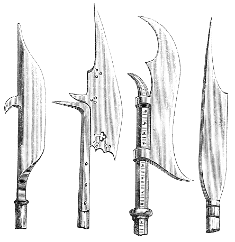
\includegraphics[scale=0.9]{Voulges}
  \end{center}

  \mylist {
    \item\mybold{Bow}  includes the shortbow and reflex bow
    \item\mybold{Club}  includes Shillelaghs, Cudgels, Bludgeons, and Batons as well as just really big, heavy sticks
    \item\mybold{Dagger}  includes the Baselard, Miséricorde, Cinquedea, and Dirk
    \item\mybold{Hand Axe}  same heads as a War-Axe, but with a short haft for throwing
    \item\mybold{Knave's Sword}  includes the Rapier and Épée
    \item\mybold{Long Sword}  includes  Sabres, Scimitars, Arming Swords, Falchions, Ulfberht, and Kopis
    \item\mybold{Mace}  includes Flanged, Pernach, and Morning Star
    \item\mybold{Military Pick}  includes both the Horseman's pick as well as a mining pick.
    \item \mybold{Polearm}  includes every polearm from 1e D\&D - the Halberd, Guisarme, Voulge, Bardiche, etc. - as well as the Lance.
}

\cbreak

\mylist {
    \item\mybold{Quarterstaff}  just a length of hardwood, sometimes with a metal tip on the end
    \item\mybold{Short Sword}  includes the Seax, Gladius, Hunting Sword, and Xiphos
    \item\mybold{Sling}  leather or rope with a pouch in it for throwing rocks.
    \item\mybold{Spear}    Go-to weapon to outfit an army for cheap.  Combines the thrusting and throwing spear.
    \item\mybold{Strongbow}  the longbow or yumi
    \item \mybold{Two-Handed sword}  includes the Zweihänder, Claymore, and Greatsword
    \item \mybold{War Axe}  includes the Archer's Axe, Dane Axe, Pollaxe and Tomahawk with a long haft 
    \item\mybold{Warhammer}  includes the Maul, Sledgehammer, and Ice Axe


  }



\newpage
\end{multicols}

\mysection{Armor}{gear-armor}

\myhighlight{The Armor \UD}{gear-armor-ud} 

Armor has a \UD that can absorb physical damage for you in \mylink{Combat}{combat}.  The first time your armor moves \DCDOWN, reduce its Current (not \MAX) \UD.  Every time thereafter, reduce \mybold{both} the Current \myital{and} \MAX \UD. Put another way - your Armor should either be equal to \MAX, or 1 die on the dice chain below it.

  \myhighlight{Repairing Armor}{gear-armor-repair}
  
  Restoring your Armor to its \MAX \UD requires a Leatherworker (Light Armor) or Smith (Medium or Heavy Armor).  Not all Settlements have a Leatherworker and/or Blacksmith - see the section on \mylink{Services}{civilization-services} under Civilization.

  Civilizations that do have a Leatherworker or Smith will cost you:  25\FE per \UD of Light Armor repaired; 25\AG per \UD of Medium Armor repaired; and 10\AU per \UD of Heavy Armor repaired.  Again, this is \myital{per} \UD.  If you had Heavy Armor with a d8 \MAX, it would cost you 20\AU to fix it properly - 10 \AU to go from d8 to d10, and another 10 to go from d10 to d12.


\hrulefill

  \mytable{X X X X X}{
    \thead{Weight} & \thead{\UD} & \thead{\MD} & \thead{Fumble Die}  &  \thead{Burden} \\
  }{
    Light  & d4 & d12 & d4  & 1 \\
    Medium  & d8 & d8 & d8  & 2 \\
    Heavy  & d12 & d4 & d12 & 3 \\
    Helmet  & - & - & +1 & n/a \\
    Shield  & - & - & +1 & 1 \\
  }




\begin{multicols}{2}
  


    \mylist {
      \item \mybold{None}  includes wizard's robes with stars and moons, filthy rags, and two-slat loincloths
      \item \mybold{Light}   includes Quilted, Cuir Bouilli, Leather, Gambeson, and Hide
      \item\mybold{Medium}  includes Chain mail,  Scaled mail, Lamellar, and Ring armorm
      \item\mybold{Heavy}  includes  Plated Mail, Coat of Plates, Splint armor, Dendra panoply, Gothic plate, and Maximilian armor
      \item\mybold{Shield}  includes round, kite, knight, buckler, targa, parma, rotella, and heater
      \item\mybold{Helmet}  includes Corinthian, galea, great helms, bacinets, frog-mouth, pickelhaubes, and armets
    }

\cbreak

    \begin{center}
  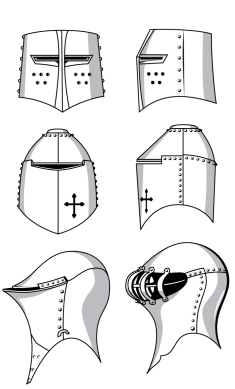
\includegraphics[scale=0.75]{Helmets}
  \end{center}



 \newpage


\end{multicols}



  \mysection{Adventuring Gear}{gear-adventuring}

  \mytable{X X X}{
    \thead{Name} & \thead{\UD}  & \thead{Burden?} \\
  }{
    25m rope &  -  & \mybold{Y}  \\
    Bandolier &  -  &  \\
    Blowpipe &  -  &  \\
    Chalk &  - &  \\
    Crowbar (Iron)&  -  & \mybold{Y}  \\
    Flask of Liquor &  d4  &  \\
    Flask of Oil &  d6  &  \mybold{Y}  \\
    Grappling Hook & - & \mybold{Y}  \\
    Grimoire (Empty)& - & \mybold{Y}  \\    
    Hand Mirror, Copper &  -  &  \\
    Lantern &  - & \mybold{Y}  \\
    Leather Work Gloves &  -  &  \\
    Matches & d10 &  \\
    Manacles &  -  &  \\
    Pipe &  - &  \\
    Provisions - Personal &  d6 & \mybold{Y}  \\
    Provisions - Journey & d4 & \mybold{Y}  (25) \\
    Quiver of Arrows/Bolts &  d10  & \mybold{Y}  \\
    Shovel &  -  & \mybold{Y}  \\
    Spikes and Hammer &  d6 & \mybold{Y}  \\
    Syringe &  d3  &  \\
    Torches and Tinderbox &  d10 & \mybold{Y}  \\
  }



    \begin{center}
  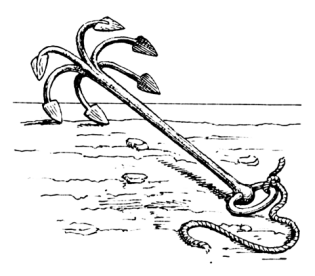
\includegraphics{GrapplingHook}
  \end{center}

\newpage



\begin{multicols}{2}


  \mybold{25m of rope} Holds 1 person and their gear safely (~100kg). The rope will break if it is put under heavier loads, impacts, or shearing (such as sawing it back and forth along a jagged lip) on an x-in-6 chance (the "x" can is up to the Arbiter)
  
  \mybold{Bandolier} You can carry 4 daggers and/or hand axes on a bandolier and it only counts as 1 Significant Item. You can't wear more than 2 bandoliers.
  
  \mybold{Blowpipe} Useful for blowing powders into people's noses.  Witches and Knaves are fans (so are Pooka, but for different reasons)
  
  \mybold{Chalk} Like school back in the day, maybe you want to play hopscotch
  
  \mybold{Crowbar} Turns most doors from a question to "can we open this door?" to "how long will it take us to open this door?"
  
  \mybold{Flask of Liquor} Just a bunch of booze. Good for rousing people and making friends. If you drink it during a Breather, you can restore 1 Grit up to your \MAX for each time you roll the \UD - but you also get 1 point of Drunk.
  
  \mybold{Flask of Oil} In a lantern, burns for 4 hours. As a molotov cocktail, can be used as a Thrown weapon that has  \mylink{Burst}{gear-weapon-burst}.  Oil burns for d4 damage for d4 Moments. Alternatively, can create a line of fire across a 3m hallway. Jumping over fire requires you to \RO using \MD+\DEX, and in the case of animals, a Morale check. 
  
  \mybold{Grappling Hook} A necessity for those hard to reach places
  
  \mybold{Grimoire (empty)} Holds 10 spells. Built to resist water and fire.

\cbreak
  
  \mybold{Hand Mirror,  Copper} Good for seeing around corners, and entirely anachronistic. Don't worry about it. But if you want to use a mirror to petrify a medusa,  you'll need a higher quality mirror than this little dinky shit.
  
  \mybold{Lantern} Holds oil and burns it so you can see.
  
  \mybold{Leather Work Glove} Allows Spriggan to touch iron
  
  \mybold{Matches} We can't all be super cool wizards who light their pipes with a snap of the fingers.  Provides a few Moments of light.
  
  \mybold{Manacles} For handcuffing people.  Reasons vary.
  
  \mybold{Provisions - Personal} The "iron rations" of the old days.  Food and water for one person

  \mybold{Provisions - Journey} Enough food and water to feed 5-7 people and 1 mount for 1 Leg of a Journey (5-10 Days).  Counts as 25 Significant Items (about 100kg).
  
  \mybold{Quiver} Filled with arrows/bolts.  Strongbows and Bows are useless without them.
  
  \mybold{Shovel} Camp-style shovel for digging latrines.  Or graves.
  
  \mybold{Pipe} Useful for smoking things (pipeweed and narcotics). Base cost gets you a crappy corncob pipe - sweet wizard's pipes are more expensive.  Sorcerers, Witches, and (surprise!) Pooka are fans.
  
  \mybold{Spikes and Hammer} Good for spiking doors shut or crucifixions.  Hammer can't hurt anyone unless it's driving the spike into an eye or something.
  
  \mybold{Syringe} Jab narcotics or sera into someone.  Leeches and Pooka are fans.
  
  \mybold{Torches and Tinderbox} Lasts 1 hour. If you drop torches, they continue to burn.  Tinderbox included with set.





  \newpage


 \mysection{Narcotics}{gear-narcotics}

You can use a narcotic up to \MAX times a Session. If you "accidentally" take more than the \MAX, you immediately Overdose.


  \myhighlight{Addiction}{gear-narcotics-addiction}

   Every Session, check for addiction:
 
   \mylist {
     \item (a) the first time you use the narcotic and 
     \item (b) if you use the narcotic \MAX number of times (or more!). 
    }


Note that there are some narcotics with a [max] of 1 - this means you roll for Addiction twice. The Addiction roll is:

  \example {
    \mybold{Addiction} 

    \RO : \FOC + d20 + modifiers

    \myital{Don't forget Mystics add their \LVL to this roll.}    

  }

  If you fail to \RO, you are addicted.  

  Once you're addicted you must use the narcotic at the start of every Session.  During a \mylink{Vacation}{civilization-vacation} you must buy a full \UD of the narcotic (but don't add it to your inventory, you'll use it all during your vacation).  Additional \UD of narcotics can be purchased on top of these before you go back out into the wilds, of course.

  If you run out of narcotics you are \mylink{Sickened}{effect-sickened} until you get the drug again.  This can be mitigated by Leechcraft. The only way to cure Addiction is to take a Vacation and gain the help of a Leeches' Medicinals\footnotemark.  When you recover from Addiction you will have the Complication listed under Recovery.

   \myhighlight{Overdose}{gear-narcotics-overdose}

  Of you exceed the \MAX listed for the narcotic, you may suffer an Overdose.  \RS using your \VIG - if you Fail, you overdose.  You are immediately afflicted as if you had imbibed a Gold (d12) Toxin\footnotemark[\value{footnote}].

  \cbreak

  \myhighlight{Common Narcotics}{gear-table-common-narcotics}

  \myital{Leeches can create brews, sera, powders, etc that are also narcotic.\footnotemark[\value{footnote}]}

  \footnotetext{See the Bell, Book, and Candle PDF}

  The costs listed get you d4 \UD of "the stuff".  See the section on \mylink{adding and splitting \UD}{arbiter-miscellania-splitting-ud} if you wish to buy multiple doses.

  \mytable{X X c}{
    \thead{d12} & \thead{Name} & \thead{\MAX} \\
  }{
    1 & Adonis & 2  \\
    2 & Black Lotus & 1  \\
    3 & Blackthroat & 2  \\
    4 & Corpse Salt & 2  \\
    5 & Dust & 1   \\
    6 & Locus & 2  \\
    7 & Pipeweed & 4 \\
    8 & Smokes & 4  \\
    9 & Twitch & 3 \\
    10 & Weed of Hasheeshian &  2    \\
    11 & Woad & 3   \\
    12 & Yellow Opium & 1  \\
}

  \myhighlight{Adonis}{gear-narcotics-adonis}

  Pheromones emitted by decaying Orchidmen, harvested by virgins and mixed with olive oil.  Makes you look and feel like a supermodel, so it's supremely expensive.  Rub the oil on your naked body and gain d6 Grit OR restore 1 \UD of Presence (up to \MAX).

  \mybold{Recovery:}  you will always be haunted by your fallen beauty - your \MAX Sanity is \DCDOWN.

  \myhighlight{Black Lotus}{gear-narcotics-black-lotus}

  The dried petals of the Black Lotus, which grows near Chaos cracks and in the labs of magical experiments gone awry. Extremely illegal, very expensive, highly addictive.  Chewing slowly (if it's the good stuff) allows a Mystic to restore 1 Blood \POOL.

  \mybold{Recovery:}  the Lotus extracts a physical toll.  Your \MAX \VIG is \DCDOWN.


  \begin{center}
  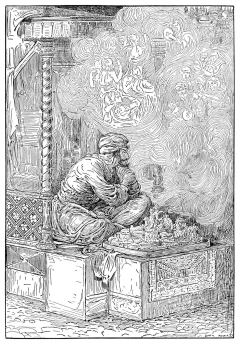
\includegraphics{Narcotics}
  \end{center}


  \myhighlight{Blackthroat}{gear-narcotics-blackthroat}

  A tar taken from the hulls of ships that sail between the isles of the Lost Cities; rubbed on the throat. You're immune to any poison you might eat or drink (Overdosing doesn't count!) for the rest of the Session. Restore 1 \UD of Talent (up to \MAX)

  \mybold{Recovery:}   Creates black sores on the neck and throat - your voice is raspy and \MAX Presence is \DCDOWN.


  \myhighlight{Corpse Salt}{gear-narcotics-corpse-salt}

  A chemical distillation of putrefying human flesh, dried to a powder and insufflated. Adds the corpse's wisdom to your own.  All \INT rolls are +2 for the rest of the Session. Philosophers can reset their Knowledge penalty.

  \mybold{Recovery:}   Hard to remember whose memories are whose.  Your \MAX \FOC is \DCDOWN.

    \myhighlight{Dust}{gear-narcotics-dust}

    The dried blood of those wounded in battle, mixed with herbs and ground to a fine powder.  Insufflated.  All \VIG rolls are +2 for the rest of the Session. Sellswords can restore 1 \UD of their Deed die.

   \mybold{Recovery:}  Your confidence in battle takes a hit (no pun intended).  Lose d6 Grit permanently.


  \myhighlight{Locus}{gear-narcotics-locus}

  The waste product of the glass beetles of the Ultraviolet Grasslands, insufflated.  Locus gives you extraordinary concentration.  All \FOC rolls are +2 for the rest of the Session.  Restore 1 \UD of Awareness (up to \MAX).

  \mybold{Recovery:}  Turns out the beetle dust does something to your kismet.   Your \MAX Talent is \DCDOWN.


  \myhighlight{Pipeweed}{gear-narcotics-pipeweed}

  A variety of weeds, harvested, cured, and smoked (in a pipe, of course). Choose 1 every time you smoke: (1) blow out beautiful smoke rings and waft them wherever you please; (2) scare away all Nearby mundane insects; (3) re-roll a failed attempt to recall something (Listen) or understand something (Lore); (4) gain +2 on any non-physical Skill \RO attempt.  You can only perform 1 effect at a time.  

  \mybold{Recovery:}   Your teeth are badly stained and your breath smells.


  \myhighlight{Smokes}{gear-narcotics-smokes}

  Most common and widely used narcotic, made from a single plant, harvested and cured, rolled in smokable paper and sold in bundles.  If you smoke during a Breather, gain 1 Grit.  Additionally, if you smoke when you are Hung Over, \RS : d6.  If you succeed, the Hung Over effect ends.

  \mybold{Recovery:}  Your teeth are badly stained and your breath smells.  

 \myhighlight{Twitch}{gear-narcotics-twitch}

  A liquid distilled from the brainstems of dead Pooka (allegedly).  Injected; syringe required.  +1 to \DEX, Init, and Fumble rolls

  \mybold{Recovery:}  yeah ... maybe there's some truth to that Pooka thing?  Your luck doesn't seem to be the same.  You take a -2 penalty on your \DEATH rolls

  \myhighlight{Weed of Hasheeshian}{gear-narcotics-weed}

  Sticky, pungent herb that gives you a minor form of telepathy.  You're immune to Surprise (including The Drop) for the rest of the Session.  Knaves and Pooka restore 1 \UD of their Luck die.

  \mybold{Recovery:}  A little slow on the uptake.  You always lose the first Init roll when you enter Combat.


  \myhighlight{Woad}{gear-narcotics-woad}

  Hallucinogenic blue paste rubbed on the face, bestows visions of the eternal battles of Valhalla, shield maidens urge you toward glory.  If you are Dying, you gain +4 to your Fight \RO and \DEATH rolls. The Woad is highly water soluble and needs to be reapplied after every Combat (presumably during a Breather) or if you get wet.  You can only have 1 application of Woad on at a given time.

  \mybold{Recovery:}  You fear losing control again.  You can't use the Combat Maneuver : Rage without making an \RS : Sanity.

\cbreak

  \myhighlight{Yellow Opium}{gear-narcotics-yellow-opium}

  The "common" opium (there are rumored to be many more in the lands of Yoon Suin), sweet smelling, haunting blue smoke in the shape of ghosts when smoked.  They whisper the truth of \TheAuthority to you.  Restore 1 \UD of Sanity (up to \MAX).  Mystics restore 1 \UD of Grace.

  \mybold{Recovery:}  Things are a little hazy now.  Your \MAX Awareness is \DCDOWN.

  \newpage


 
  \mysection{Transport}{gear-transport}

  \begin{center}
  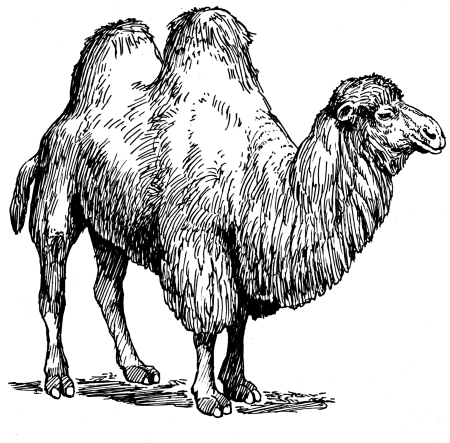
\includegraphics{Camel}
  \end{center}

   
  \mybold{Mule}: basic beast of burden, doesn't panic easily.  Can carry about 100kg (25 \mylink{Significant Items}{equipment-significant-items})

  \mybold{Horse}:   good for riding, tends to bolt when scared.  Can carry about 200kg (50 \mylink{Significant Items}{equipment-significant-items})

  \mybold{Camel}:  never runs, generally an asshole, only found in desert terrain.  Can carry about 250kg (62 \mylink{Significant Items}{equipment-significant-items})

  \mybold{Push cart}:  push around all your stuff, takes 2 hands to use.  Can hold about 50kg worth of stuff (12 \mylink{Significant Items}{equipment-significant-items})

  \mybold{Wagon}:  can't go anywhere on its own.  Depending on the size, can carry 100 - 400kg worth of gear and people (roll a d4 to see how big the one available might be).  Needs appropriate number of mounts to pull it (100kg = 1 mule, 200kg = 2 mules or a horse, etc.)

  \mybold{Rowboat}:  only available near civilizations with water.  Same weight rules as wagons (100 - 400kg worth of gear and people).

\cbreak      

    \myhighlight{Mount Morale}{gear-mount-morale}
    
    Mounts must pass a \mylink{Morale}{monster-morale} check to enter dangerous situations (combat, entering a dungeon, jumping a chasm, etc). Random mounts have Cowardly morale; trained mounts (warhorses, etc.) have Orderly morale.  If the morale check fails the mount will take no action (though if you want to flee on your mount, that's allowed). If your mount fails a Morale check, you can roll a \mylink{Skill:Travel}{skill-travel} check.  If you succeed, they get another morale check. You can \mylink{Bum Rush}{combat-deeds-bum-rush} while mounted.  If you or your mount take damage while mounted, you can make a Skill:Travel check and decide who takes the damage (you or the mount)


  \mysection{Henchmen}{gear-henchmen}

    \setcounter{footnote}{0}
    \myital{Based on Arnold Kemp's article}\footnote{\url{https://goblinpunch.blogspot.com/2020/04/dungeoncrawling-hirelings.html}{}}

    \mysubsection{Loyalty Checks}{gear-henchmen-loyalty-checks}

    A Loyalty Check works the same way as \mylink{Monster Morale}{monster-morale} i.e. roll 2d6, if the number is greater than (but not equal to) the henchmen's Loyalty, they'll refuse to do what you're trying to coax them into doing.  If you wish, you can roll your Presence \UD and add it to the Henchmen's Loyalty, but a) you have to do it before you roll 2d6; b) it only counts for that Loyalty check;  and c) if you roll a Failure (a 1 or a 2), the Henchman automatically refuses, and their Loyalty goes down by 1.

    Asking a hireling to take more risks than the rest of the party causes them to lose 1 Loyalty, regardless of whether or not they accept or refuse. Good treatment can make their Loyalty go up (to a maximum of 11).  Poor treatment obviously can drop it.

    If a henchmen ever hits 0 Loyalty, they'll try to escape as soon as possible.  Maybe with your stuff.  Maybe they'll try to kill you, too.


    \mysubsection{Hirelings}{gear-hirelings}

    Hirelings will generally work for a set rate, usually 5 coins/day.  If a fight breaks out, they run for cover. They'll refuse to do anything overtly risky, but can be coaxed into doing something with minor risk with a Loyalty check.  Overtly risky tasks might be being the first one down a hallway, or pulling an unmarked lever. Moderately risky tasks might standing watch in the hall while the party is in a room.

    Hirelings have a starting Loyalty of 3.

    \myhighlight{Linkboys}{gear-hirelings-linkboys}

    Linkboys hold torches so you don't have to. They only have a 1-in-6 chance of a torch going out if they should drop one for any reason, and they are able to light a torch using one action.  Torches not included.

    \myhighlight{Porters}{gear-hirelings-porters}

    Beefy numbskulls hired to carry your stuff. They can carry 10 \mylink{Significant Items}{equipment-significant-items} worth of gear.

    \myhighlight{Guides}{gear-hirelings-guides}

    Guys who know how to get to somewhere specific. Useful if you're \mylink{Traveling}{arbiter-travel} off the beaten track. Guides are Skilled (d12) in Travel, but only to a specific location.

    \myhighlight{Cook}{gear-hirelings-cook}

    Good to have on \mylink{long journeys}{arbiter-travel}.  If you ever need to roll your Party Provisions, the Cook is Skilled (d12) in Travel, but only when it comes to food.

    \cbreak

    \mysubsection{Mercenaries}{gear-mercenaries}

    Mercenaries will work for a half share of money, or for 10 coins a day (whatever is highest).  A mercenary will try to stay as close to the person who hired them as possible.  They stand in the background when possible, but don't generally shirk from combat.

    Mercenaries have a starting Loyalty of 7. They'll have to check their Loyalty if they're asked to do something overtly risky.  In combat, they'll need to check Loyalty a) when the first adventurer starts \mylink{Dying}{combat-dying}; b) when half the adventurers are incapacitated; and c) if the person they're attached to becomes incapacitated.

    \myhighlight{Meatshield}{gear-mercenary-meatshield}

    A Meatshield gives you +3 to your Fight \RO, but they don't take a combat turn themselves.  Any physical damage you would take you can put onto the Meatshield instead.  Meatshields have 6 Flesh and 0 Grit, but you can give them Armor if you like.

    \myhighlight{Trapsman}{gear-mercenary-trapsman}

    A trapsman can be coaxed into picking locks, removing traps, and scouting rooms.  They have the Tinkering skill of 3-in-6.  They give you a +1 to your Fight \RO, but they don't take a combat turn themselves.  Any physical damage you would take you can put onto the Trapsman instead.  They have 4 Flesh, 4 Grit, and can't wear any Armor.

\newpage

\end{multicols}

  \mysection{Cost}{equipment-cost}

  The costs listed below are static - sometimes you might barter for a lower price, sometimes you get ripped off - but they tend to average out to the cost shown.   Prices increase depending on the Settlement type (Gold settlements charge more for basic goods than Iron settlements), and certain equipment is generally only available in the appropriate Settlement or lower (Iron settlements only have what's listed; Silver settlements have Iron and Silver gear; and Gold settlements have everything). 

  \mytable{l X X X} {
   \thead{}  & \thead{Small/Iron} & \thead{Medium/Silver}  & \thead{Large/Gold} \\
  }{
    Armor, Heavy & \myital{n/a} & \myital{n/a} & 100 \\
    Armor, Helmet & 80 & 10 & 2 \\
    Armor, Light & 120 & 15 & 2 \\
    Armor, Medium & \myital{n/a} & 200 & 25 \\
    Armor, Shield & \myital{n/a} & 75 & 10 \\
    Gear, 25m Rope & 5 & 1 & 1 \\
    Gear, Bandolier & \myital{n/a} & 10 & 2 \\
    Gear, Chalk & 3 & 1 & 1 \\
    Gear, Crowbar & 10 & 2 & 1 \\
    Gear, Flask of Oil & \myital{n/a} & 5 & 1 \\
    Gear, Grappling Hook & \myital{n/a} & 15 & 2 \\
    Gear, Grimoire (Empty) & \myital{n/a} & \myital{n/a} & 50 \\
    Gear, Hand Mirror (Copper) & \myital{n/a} & \myital{n/a} & 5 \\
    Gear, Lantern & 20 & 3 \\
    Gear, Leather Work Gloves & 15 & 2 & 1 \\
    Gear, Liquor & varies & varies & varies \\
    Gear, Manacles & \myital{n/a} & \myital{n/a} & 10 \\
    Gear, Matches & 1 & 1 & 1 \\
    Gear, Pipe & varies & varies & varies \\
    Gear, Provisions - Journey & 200 & 25 & 4 \\
    Gear, Provisions - Personal & 25 & 4 & 1 \\
    Gear, Quiver of Arrows & 25 & 4 & 1 \\
    Gear, Shovel & 20 & 3 & 1 \\
    Gear, Spikes and Hammer & 15 & 2 & 1 \\
    Gear, Spyglass & \myital{n/a} & \myital{n/a} & 25 \\
    Gear, Syringe & \myital{n/a} & \myital{n/a} & 15 \\
    Gear, Torches and Tinder & 20 & 3 & 1 \\
    Narcotic, Adonis & \myital{n/a} & \myital{n/a} & 50 \\
    Narcotic, Black Lotus & \myital{n/a} & \myital{n/a} & 25 \\
    Narcotic, Blackthroat & \myital{n/a} & 25 & 4 \\
    Narcotic, Corpse Salt & \myital{n/a} & \myital{n/a} & 25 \\
    Narcotic, Dust & \myital{n/a} & 25 & 4 \\

}



  \mytable{l X X X} {
    \thead{}  & \thead{Small/Iron} & \thead{Medium/Silver}  & \thead{Large/Gold} \\
  }{

    Narcotic, Locus & \myital{n/a} & 25 & 4 \\
    Narcotic, Pipeweed & 5 & 1 & 1 \\
    Narcotic, Smokes & 5 & 1 & 1 \\
    Narcotic, Twitch & \myital{n/a} & 25 & 4 \\
    Narcotic, Weed of Hasheeshian & 10 & 2 & 1 \\
    Narcotic, Woad & \myital{n/a} & 10 & 2 \\
    Narcotic, Yellow Opium & \myital{n/a} & \myital{n/a} &  25 \\
    Transport, Camel & \myital{n/a} & 40 & 5 \\
    Transport, Horse & \myital{n/a} & 400 & 50 \\
    Transport, Mule & 75 & 10 & 2 \\
    Transport, Push Cart & 75 & 10 & 2 \\
    Transport, Rowboat & 200 & 25 & 4 \\
    Transport, Wagon & \myital{n/a} & 400 & 50 \\
    Weapon, Bow & 50 & 7 & 1 \\
    Weapon, Club & 5 & 1 & 1 \\
    Weapon, Dagger & 20 & 3 & 1 \\
    Weapon, Hand Axe & 30 & 4 & 1 \\
    Weapon, Knave's Sword & \myital{n/a} & \myital{n/a} & 10 \\
    Weapon, Longsword & \myital{n/a} & 40 & 5 \\
    Weapon, Mace & \myital{n/a} & 35 & 5 \\
    Weapon, Military Pick & \myital{n/a} & 30 & 4 \\
    Weapon, Polearm & \myital{n/a} & \myital{n/a} & 10 \\
    Weapon, Quarterstaff & 10 & 2 & 1 \\
    Weapon, Shortsword & \myital{n/a} & 30 & 4 \\
    Weapon, Sling & 5 & 1 & 1 \\
    Weapon, Spear & 10 & 2 & 1 \\
    Weapon, Strongbow & \myital{n/a} & 50 & 7 \\
    Weapon, Two-Handed Sword & \myital{n/a} & \myital{n/a} & 15 \\
    Weapon, War Axe & \myital{n/a} & 60 & 8 \\
    Weapon, Warhammer & 100 & 13 & 2
}

\begin{multicols}{2}





  \footnotetext{See the Bell, Book, and Candle PDF}
  \setcounter{footnote}{0}




} %end
